\documentclass[10pt,aspectratio=169]{beamer}

% Cấu hình theme
\usetheme{Madrid}
\usecolortheme{default}
\usefonttheme{professionalfonts} % Sử dụng font chuyên nghiệp hơn
\setbeamerfont{caption}{size=\scriptsize}

% Gói hỗ trợ tiếng Việt và các gói khác
\usepackage[utf8]{vietnam}
\usepackage[utf8]{inputenc}
\usepackage[T5]{fontenc}
\usepackage{lmodern} % Font Latin Modern sắc nét hơn
\usepackage[scaled]{helvet} % Dùng font Helvetica (giống Arial) làm font chính
\renewcommand{\familydefault}{\sfdefault} % Chắc chắn dùng sans-serif

\usepackage{bookmark}
\usepackage{graphicx}
\usepackage{booktabs}
\usepackage{algorithm}
\usepackage{algpseudocode}
\usepackage{listings}
\usepackage{xcolor}
\usepackage{tikz}
\usepackage{multirow}
\usepackage{array}
\usetikzlibrary{shapes,arrows,positioning,fit,calc}

% Cấu hình code block đẹp hơn

\lstset{
    language=Python,
    basicstyle=\ttfamily\scriptsize, % Tăng size lên xíu cho dễ nhìn
    keywordstyle=\color{blue}\bfseries,
    commentstyle=\color{green!50!black}\itshape, % Comment in nghiêng, màu dịu hơn
    stringstyle=\color{orange!80!black},
    identifierstyle=\color{black},
    breaklines=true,
    frame=shadowbox, % Khung bóng đổ đẹp hơn
    rulesepcolor=\color{gray},
    showstringspaces=false,
    numbers=left,
    numberstyle=\tiny\color{gray},
    numbersep=5pt,
    tabsize=4,
    backgroundcolor=\color{yellow!5}, % Nền code màu nhạt dễ đọc
    escapeinside={(*@}{@*)}
}

% Định nghĩa lại tên thuật toán
\floatname{algorithm}{Thuật toán}
\renewcommand{\algorithmicrequire}{\textbf{Input:}}
\renewcommand{\algorithmicensure}{\textbf{Output:}}

% --- ĐỊNH NGHĨA TRANG BÌA CUSTOM (MINIMALIST WHITE) ---
\setbeamertemplate{title page}{
    \begin{tikzpicture}[remember picture,overlay]
        % Thanh màu xanh mỏng ở trên cùng
        \fill[structure.fg] (current page.north west) rectangle ([yshift=-0.2cm]current page.north east);
    \end{tikzpicture}
    
    \vspace{1.5cm}
    
    % Dòng tên trường
    {\tiny\bfseries\color{structure.fg!80} TRƯỜNG ĐẠI HỌC XÂY DỰNG HÀ NỘI \\ KHOA CÔNG NGHỆ THÔNG TIN \par}
    
    \vspace{0.5cm}
    
    % Tiêu đề chính (Font Serif to, đậm - Đã giảm size theo yêu cầu)
    {\usefont{T5}{put}{b}{n}\fontsize{16}{22}\selectfont\textcolor{black}{Ứng dụng thuật toán Eclat trong phân tích hành vi người dùng qua dữ liệu clickstream để gợi ý nội dung}\par}
    
    \vspace{0.3cm}
    
    % Subtitle
    {\color{gray} Báo cáo Bài tập lớn môn Khai phá dữ liệu \par}
    
    \vspace{1.5cm} 
    
    % Cột thông tin (Giảng viên & Sinh viên)
    \begin{columns}[t]
        \column{0.45\textwidth}
            {\scriptsize\bfseries\color{structure.fg} GIẢNG VIÊN HƯỚNG DẪN}\\[0.1cm]
            {\large\bfseries TS. Phạm Hồng Phong}
            
        \column{0.55\textwidth}
            {\scriptsize\bfseries\color{structure.fg} NHÓM THỰC HIỆN}\\[0.1cm]
            {\small
            1. Nguyễn Việt Anh (0203968)\\
            2. Nguyễn Việt Hùng (0208768)\\
            3. Đỗ Quang Hợp (0208568)
            }
    \end{columns}
    
    \vfill
}

% Thông tin Metadata
\title[Thuật toán Eclat]{Ứng dụng thuật toán Eclat trong phân tích hành vi\\người dùng qua dữ liệu clickstream để gợi ý nội dung}

\author[Việt Anh - Việt Hùng - Quang Hợp]{
    Nguyễn Việt Anh \and Nguyễn Việt Hùng \and Đỗ Quang Hợp
}
\institute[ĐH Xây Dựng HN]{
    Khoa Công nghệ Thông tin \\
    Trường Đại học Xây Dựng Hà Nội
}
\date{Tháng 2 năm 2026}

\begin{document}

% Slide 1: Trang bìa
\begin{frame}
    \titlepage
\end{frame}

% Slide 2: Mục lục
\begin{frame}{Nội dung trình bày}
    \tableofcontents
\end{frame}

% ============================================================
% CHƯƠNG 1: TỔNG QUAN
% ============================================================
\section{Tổng quan đề tài}

\begin{frame}{Đặt vấn đề}
    \textbf{Bối cảnh thực tế:}
    \begin{itemize}
        \item Sự bùng nổ dữ liệu hành vi người dùng (clickstream data) trên các website/ứng dụng.
        \item Phân tích dữ liệu này giúp: Hiểu hành vi người dùng, tối ưu UX, tăng doanh thu.
    \end{itemize}

    \vspace{0.5cm}
    \textbf{Giải pháp - Khai phá luật kết hợp:}
    \begin{itemize}
        \item Tìm kiếm các mối quan hệ tiềm ẩn giữa các mục trong tập dữ liệu lớn.
        \item Ví dụ kinh điển: "Bia và Tã lót".
    \end{itemize}
\end{frame}

\begin{frame}{Mục tiêu đề tài}
    \begin{enumerate}
        \item \textbf{Nghiên cứu \& Triển khai}: Thuật toán \textbf{Eclat} từ đầu (from scratch), không dùng thư viện có sẵn.
        \item \textbf{Ứng dụng thực tế}: Phân tích dữ liệu clickstream từ \textbf{MSNBC.com} (gần 1 triệu giao dịch).
        \item \textbf{Sinh luật gợi ý}: Dạng \textit{"Nếu xem A $\rightarrow$ Gợi ý B"}.
        \item \textbf{Đánh giá}: Sử dụng các chỉ số Support, Confidence, Lift.
    \end{enumerate}
\end{frame}

\begin{frame}{Phạm vi nghiên cứu}
    \begin{itemize}
        \item \textbf{Dữ liệu}: MSNBC.com Anonymous Web Data (UCI Machine Learning Repository).
        \item \textbf{Thuật toán}: Eclat (Equivalence Class Transformation) [Zaki, 2000].
        \item \textbf{Công nghệ}: Python 3.x.
        \item \textbf{Phương pháp}: Cài đặt thủ công cấu trúc dữ liệu và giải thuật.
    \end{itemize}
\end{frame}

% ============================================================
% CHƯƠNG 2: CƠ SỞ LÝ THUYẾT
% ============================================================
\section{Cơ sở lý thuyết}

\begin{frame}{Khai phá luật kết hợp}
    \begin{block}{Các khái niệm cơ bản}
        \begin{itemize}
            \item \textbf{Itemset (Tập mục)}: Tập hợp các mục, ví dụ $X = \{A, B\}$.
            \item \textbf{Support (Độ hỗ trợ)}: Tỷ lệ xuất hiện của itemset trong CSDL.
            \[ Support(X) = \frac{|\{T \in D : X \subseteq T\}|}{|D|} \]
            \item \textbf{Frequent Itemset}: Itemset có $Support \geq min\_support$.
            \item \textbf{Luật kết hợp}: $X \Rightarrow Y$ ("Nếu $X$ thì $Y$").
        \end{itemize}
    \end{block}
\end{frame}

\begin{frame}{Các chỉ số đánh giá luật}
    \begin{columns}[t]
        \column{0.5\textwidth}
            \textbf{1. Confidence (Độ tin cậy)}
            \[ Conf(X \Rightarrow Y) = \frac{Sup(X \cup Y)}{Sup(X)} \]
            \begin{itemize}
                \item Xác suất có điều kiện $P(Y|X)$.
                \item Đo lường độ "chắc chắn" của luật.
            \end{itemize}
        
        \column{0.5\textwidth}
            \textbf{2. Lift (Độ tương quan)}
            \[ Lift = \frac{Sup(X \cup Y)}{Sup(X) \times Sup(Y)} \]
            \begin{itemize}
                \item $>1$: Tương quan dương (Tốt).
                \item $=1$: Độc lập.
                \item $<1$: Tương quan âm.
            \end{itemize}
    \end{columns}
\end{frame}

% --- VÍ DỤ MINH HỌA THEO BÁO CÁO ---


\begin{frame}{Thuật toán Eclat: Tổng quan}
    \textbf{Eclat} (Equivalence Class Transformation)
    \begin{itemize}
        \item Đề xuất: \textbf{Mohammed J. Zaki} (2000).
        \item Là thuật toán khai phá tập phổ biến (Frequent Itemset Mining) hiệu quả cao.
        \item \textbf{Tư tưởng chính:} Thay vì đếm số lần xuất hiện (như Apriori), Eclat sử dụng \textbf{giao của các tập định danh giao dịch (Intersection of TID-Sets)}.
    \end{itemize}
    
    \vspace{0.5cm}
    \textbf{Chiến lược tìm kiếm:}
    \begin{enumerate}
        \item \textbf{Vertical Data Format}: Chuyển đổi dữ liệu sang dạng dọc.
        \item \textbf{DFS (Depth-First Search)}: Duyệt theo chiều sâu để tìm tập phổ biến.
    \end{enumerate}
\end{frame}

\begin{frame}{Định dạng dữ liệu (Data Format)}
    \begin{columns}[t]
        \column{0.48\textwidth}
            \textbf{A. Horizontal Format (Truyền thống)}
            \begin{table}\centering\scriptsize
            \begin{tabular}{|c|l|}
            \hline \textbf{TID} & \textbf{Items} \\ \hline
            1 & A, B, C \\
            2 & A, B \\
            3 & A, C \\
            \hline \end{tabular}
            \end{table}
            
            \begin{alertblock}{Vấn đề}
                Để biết \textbf{\{A, B\}} xuất hiện bao nhiêu lần:
                \begin{itemize}
                    \item Phải quét từng dòng (Scan DB).
                    \item Kiểm tra: Dòng 1 có A, B? (Có) $\rightarrow$ +1.
                    \item Dòng 2 có A, B? (Có) $\rightarrow$ +1.
                \end{itemize}
                $\Rightarrow$ \textbf{Rất tốn kém (Expensive Scans)}.
            \end{alertblock}
        
        \column{0.48\textwidth}
            \textbf{B. Vertical Format (Eclat)}
            \begin{table}\centering\scriptsize
            \begin{tabular}{|c|l|}
            \hline \textbf{Item} & \textbf{TID-Set (Ai mua?)} \\ \hline
            A & \{1, 2, 3\} \\
            B & \{1, 2\} \\
            C & \{1, 3\} \\
            \hline \end{tabular}
            \end{table}
            
            \begin{exampleblock}{Giải pháp của Eclat}
                Để biết \textbf{\{A, B\}} xuất hiện bao nhiêu lần:
                \begin{itemize}
                    \item Lấy TID(A) giao TID(B).
                    \item $\{1,2,3\} \cap \{1,2\} = \{1,2\}$.
                    \item Đếm kích thước = 2.
                \end{itemize}
                $\Rightarrow$ \textbf{Tính toán tức thì (Instant Calculation)}.
            \end{exampleblock}
    \end{columns}
\end{frame}

\begin{frame}{Nguyên lý hoạt động cốt lõi}
    \begin{columns}
        \column{0.5\textwidth}
        \textbf{Cơ sở toán học:}
        \begin{itemize}
            \item Eclat dựa trên lý thuyết tập hợp (Set Theory).
            \item Thay vì \textit{kiểm tra} từng giao dịch xem có chứa A và B không (Scan), ta \textit{xác định} giao dịch đó bằng cách lấy phần chung của tập TID.
            \item \textbf{Định lý}: Tập hợp các giao dịch chứa itemset $X \cup Y$ chính là giao của tập TID chứa $X$ và tập TID chứa $Y$.
            \[ TID(XY) = TID(X) \cap TID(Y) \]
        \end{itemize}

        \column{0.5\textwidth}
        \centering
        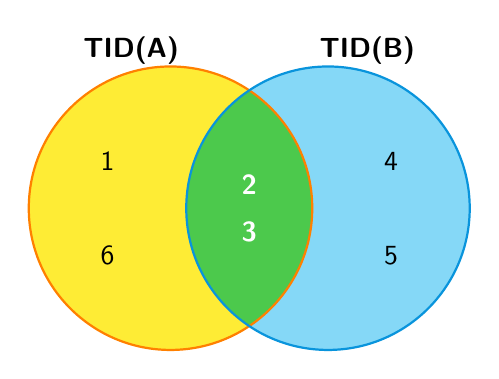
\begin{tikzpicture}[thick]
            % Tô màu Vòng tròn A (Vàng) - Nguyên khối
            \fill[yellow!90!orange, opacity=0.8] (-1,0) circle (1.8cm);
            
            % Tô màu Vòng tròn B (Xanh Cyan) - Nguyên khối
            \fill[cyan!60, opacity=0.8] (1,0) circle (1.8cm);

            % Tô lại màu phần giao (Xanh lá) 
            % Dùng clip để chỉ tô phần giao nhau
            \begin{scope}
                \clip (-1,0) circle (1.8cm);
                \fill[green!70!black!70] (1,0) circle (1.8cm);
            \end{scope}

            % Vẽ viền 2 vòng tròn (Vẽ sau cùng để đè lên màu tô)
            \draw[orange, thick] (-1,0) circle (1.8cm);
            \draw[cyan!80!blue, thick] (1,0) circle (1.8cm);

            % Label
            \node at (-1.5, 2) {\textbf{TID(A)}};
            \node at (1.5, 2) {\textbf{TID(B)}};

            % Nội dung bên trong (Số) - Căn chỉnh vị trí để không bị lẹm vào phần giao
            \node at (-1.8, 0.6) {1};
            \node at (-1.8, -0.6) {6};
            
            \node at (1.8, 0.6) {4};
            \node at (1.8, -0.6) {5};

            % Phần giao (Màu chữ trắng)
            \node at (0, 0.3) {\textbf{\textcolor{white}{2}}};
            \node at (0, -0.3) {\textbf{\textcolor{white}{3}}};
        \end{tikzpicture}
        \\
        \footnotesize \textit{Màu xanh lá thể hiện tập giao nhau (Intersection)}
    \end{columns}
    
    \vspace{0.2cm}
    \textbf{Kết luận từ hình:}
    \begin{itemize}
        \item $TID(A) = \{1, 2, 3, 6\}$ (Có 4 phần tử $\rightarrow$ \textbf{Sup=4})
        \item $TID(B) = \{2, 3, 4, 5\}$ (Có 4 phần tử $\rightarrow$ \textbf{Sup=4})
        \item $\rightarrow TID(A \cap B) = \{\textbf{2, 3}\}$ (Còn 2 phần tử $\rightarrow$ \textbf{Sup=2})
    \end{itemize}
    \textit{*Sup (Support Count): Số lượng giao dịch chứa item.}
\end{frame}

\begin{frame}{3. Quy trình thực hiện (Workflow)}
    \begin{enumerate}
        \item \textbf{Bước 1: Khởi tạo \& Chuyển đổi (Initialization)}
        \begin{itemize}
            \item Quét CSDL một lần để chuyển sang dạng dọc (Vertical Format).
            \item Lọc bỏ các item không phổ biến ($Support < min\_sup$).
        \end{itemize}
        
        \item \textbf{Bước 2: Sắp xếp (Sorting)}
        \begin{itemize}
            \item Sắp xếp các item theo tần suất tăng dần để tối ưu duyệt cây.
        \end{itemize}

        \item \textbf{Bước 3: Giao tập TID (Intersection)}
        \begin{itemize}
            \item Tính toán Support bằng phép giao: $TID(XY) = TID(X) \cap TID(Y)$.
        \end{itemize}
        
        \item \textbf{Bước 4: Tìm kiếm chiều sâu (DFS)}
        \begin{itemize}
            \item Nếu Support $\ge min\_sup$ $\rightarrow$ Lưu kết quả và tiếp tục đệ quy.
            \item Nếu Support $< min\_sup$ $\rightarrow$ Cắt tỉa nhánh (Pruning).
        \end{itemize}
        
        \item \textbf{Bước 5: Quay lui (Backtrack)}
        \begin{itemize}
            \item Quay lại nhánh cha khi nhánh con đã thám hiểm hết.
        \end{itemize}
    \end{enumerate}
\end{frame}




% --- Slide Mã giả & Ví dụ minh họa (Moved here) ---

\begin{frame}[fragile]{Mã giả thuật toán Eclat}
    \scriptsize
    \begin{algorithmic}[1]
        \State \textbf{Input:} $DB$ (Cơ sở dữ liệu), $min\_sup$ (Ngưỡng \%)
        \State \textbf{Output:} $F$ (Danh sách tập phổ biến)
        
        \State $min\_count \gets |DB| \times min\_sup$
        \State $Items \gets$ Chuyển $DB$ sang dạng dọc (Item $\to$ TIDs)
        \State Lọc bỏ các Item có $|TIDs| < min\_count$
        \State Sắp xếp $Items$ theo tần suất giảm dần
        \State \Call{EclatDFS}{$\emptyset, Items, min\_count$}
        \State \Return $F$
        
        \Procedure{EclatDFS}{$Prefix, CurrentItems, min\_count$}
            \ForAll{$(i, T_i) \in CurrentItems$}
                \State $NewPattern \gets Prefix \cup \{i\}$
                \State Thêm $(NewPattern, |T_i|)$ vào $F$
                
                \State $SuffixItems \gets \emptyset$
                \ForAll{$(j, T_j) \in CurrentItems$ với $j > i$}
                    \State $T_{new} \gets T_i \cap T_j$ \Comment{Giao tập TID}
                    \If{$|T_{new}| \ge min\_count$}
                        \State Thêm $(j, T_{new})$ vào $SuffixItems$
                    \EndIf
                \EndFor
                
                \If{$SuffixItems \neq \emptyset$}
                    \State \Call{EclatDFS}{$NewPattern, SuffixItems, min\_count$}
                \EndIf
            \EndFor
        \EndProcedure
    \end{algorithmic}
\end{frame}

\section{Ví dụ minh họa thuật toán}

\begin{frame}{Ví dụ minh họa thuật toán}
    \textbf{Bước 0: Xác định ngưỡng đếm (Min Support Count)}
    \[ min\_count = \lceil |D| \times min\_support \rceil = \lceil 4 \times 0.5 \rceil = 2 \]
    $\Rightarrow$ Loại bỏ itemset xuất hiện dưới 2 lần (Pruning).

    \vspace{0.2cm}
    \textbf{Input (Horizontal Format)}
    \begin{table}\centering\scriptsize
    \begin{tabular}{|c|l|}
    \hline \textbf{TID} & \textbf{Items} \\ \hline
    1 & A, B, C \\
    2 & B, C, D \\
    3 & A, C, D \\
    4 & A, B, D \\
    \hline \end{tabular}
    \end{table}

    \vspace{0.2cm}
    \textbf{Bước 1: Chuyển đổi sang Vertical Format}
    (Tạo danh sách TID-Sets và Sắp xếp A, B, C, D)
    \begin{table}\centering\scriptsize
    \begin{tabular}{|c|l|c|}
    \hline \textbf{Item (Suffix)} & \textbf{TID-Set} & \textbf{Status} \\ \hline
    A & \{1, 3, 4\} (3) & $\ge$ 2 (Giữ) \\
    B & \{1, 2, 4\} (3) & $\ge$ 2 (Giữ) \\
    C & \{1, 2, 3\} (3) & $\ge$ 2 (Giữ) \\
    D & \{2, 3, 4\} (3) & $\ge$ 2 (Giữ) \\
    \hline \end{tabular}
    \end{table}
    \centering\footnotesize \textit{Sắp xếp items theo tần suất hoặc từ điển (A, B, C, D).}
\end{frame}

\begin{frame}{Ví dụ minh họa thuật toán}
    \textbf{Bước 2: Mở rộng nhánh A} \\
    \textbf{Quy trình:} Lấy \textbf{A} làm Prefix (tiền tố). Kết hợp với các items đứng sau (Suffix: B, C, D).
    
    \begin{table}\centering\small
    \caption{Mở rộng nhánh Prefix = \{A\} (TID=\{1,3,4\})}
    \begin{tabular}{|c|l|c|l|}
    \hline
    \textbf{Suffix ($X$)} & \textbf{Phép giao: $TID(A) \cap TID(X)$} & \textbf{Count} & \textbf{Kết quả} \\
    \hline
    B & $\{1,3,4\} \cap \{1,2,4\} = \{1,4\}$ & 2 & $\ge 2 \rightarrow$ \textbf{Lấy \{A,B\}} \\
    C & $\{1,3,4\} \cap \{1,2,3\} = \{1,3\}$ & 2 & $\ge 2 \rightarrow$ \textbf{Lấy \{A,C\}} \\
    D & $\{1,3,4\} \cap \{2,3,4\} = \{3,4\}$ & 2 & $\ge 2 \rightarrow$ \textbf{Lấy \{A,D\}} \\
    \hline
    \end{tabular}
    \end{table}
    $\Rightarrow$ Danh sách ứng viên tiếp theo $L_A = [B, C, D]$.
\end{frame}

\begin{frame}{Ví dụ minh họa thuật toán}
    \textbf{Bước 3: Đệ quy sâu hơn} \\
    \textbf{Quy trình:} Từ danh sách $L_A$, tiếp tục đào sâu (DFS) với từng item làm prefix mới (ví dụ \{A,B\}).
    
    \begin{table}\centering\small
    \caption{Đào sâu tìm kiếm 3-itemsets từ nhánh A}
    \begin{tabular}{|l|c|l|c|l|}
    \hline
    \textbf{Prefix} & \textbf{Suffix} & \textbf{Phép giao TID} & \textbf{Count} & \textbf{Kết luận} \\
    \hline
    \{A,B\} & C & $\{1,4\} \cap \{1,3\} = \{1\}$ & 1 & $<2 \rightarrow$ \textbf{Loại (Pruned)} \\
    (TID=\{1,4\}) & D & $\{1,4\} \cap \{3,4\} = \{4\}$ & 1 & $<2 \rightarrow$ \textbf{Loại (Pruned)} \\
    \hline
    \{A,C\} & D & $\{1,3\} \cap \{3,4\} = \{3\}$ & 1 & $<2 \rightarrow$ \textbf{Loại (Pruned)} \\
    (TID=\{1,3\}) & & & & \\
    \hline
    \end{tabular}
    \end{table}
    $\Rightarrow$ Nhánh A không sinh ra được tập phổ biến nào kích thước $k=3$. Thuật toán quay lui (backtrack).
\end{frame}

\begin{frame}{Ví dụ minh họa thuật toán}
    \textbf{Bước 4 \& 5: Các nhánh còn lại (B, C)} \\
    Sau khi xử lý xong A, xét tiếp nhánh B và C.
    
    \begin{table}\centering\small
    \caption{Mở rộng các nhánh B và C}
    \begin{tabular}{|l|c|l|c|l|}
    \hline
    \textbf{Prefix} & \textbf{Suffix} & \textbf{Phép giao TID} & \textbf{Count} & \textbf{Kết quả} \\
    \hline
    \textbf{\{B\}} & C & $\{1,2,4\} \cap \{1,2,3\} = \{1,2\}$ & 2 & $\ge 2 \rightarrow$ \textbf{Lấy \{B,C\}} \\
    (TID=\{1,2,4\}) & D & $\{1,2,4\} \cap \{2,3,4\} = \{2,4\}$ & 2 & $\ge 2 \rightarrow$ \textbf{Lấy \{B,D\}} \\
    \hline
    \multicolumn{5}{|c|}{\textit{Thử đào sâu từ \{B,C\}: $\{1,2\} \cap \{2,4\} = \{2\}$ (Count=1) $\rightarrow$ Loại}} \\
    \hline
    \textbf{\{C\}} & D & $\{1,2,3\} \cap \{2,3,4\} = \{2,3\}$ & 2 & $\ge 2 \rightarrow$ \textbf{Lấy \{C,D\}} \\
    (TID=\{1,2,3\}) & & & & \\
    \hline
    \end{tabular}
    \end{table}
\end{frame}

\begin{frame}{Ví dụ minh họa thuật toán}
    \textbf{Tổng kết kết quả}
    Sau khi duyệt hết toàn bộ không gian, ta thu được bảng tổng hợp:
    
    \begin{table}\centering
    \begin{tabular}{|c|l|c|l|}
    \hline \textbf{Kích thước} & \textbf{Frequent Itemsets} & \textbf{Slg} & \textbf{Ghi chú} \\ \hline
    k=1 & \{A\}, \{B\}, \{C\}, \{D\} & 4 & Support = 3 (75\%) \\ \hline
    \multirow{2}{*}{k=2} & \{A,B\}, \{A,C\}, \{A,D\} & \multirow{2}{*}{6} & \multirow{2}{*}{Support = 2 (50\%)} \\
                         & \{B,C\}, \{B,D\}, \{C,D\} & & \\ \hline
    k=3 & \textit{(Không tìm được)} & 0 & Bị cắt tỉa (Pruned) \\ \hline
    \textbf{Tổng} & \textbf{Tổng số tập phổ biến} & \textbf{10} & \\ \hline
    \end{tabular}
    \end{table}
    
    \textbf{Kết luận:} Eclat tìm ra chính xác tất cả các tập phổ biến mà \textbf{không cần quét lại CSDL gốc}.
\end{frame}

% ============================================================
% CHƯƠNG 3: DỮ LIỆU VÀ TIỀN XỬ LÝ
% ============================================================
\section{Dữ liệu và Tiền xử lý}

\begin{frame}{Giới thiệu bộ dữ liệu MSNBC}
    \begin{itemize}
        \item \textbf{Nguồn}: UCI Machine Learning Repository.
        \item \textbf{Thời gian}: 28/09/1999 từ MSNBC.com.
        \item \textbf{Thống kê}:
        \begin{itemize}
            \item Tổng số phiên: \textbf{989,818}.
            \item Số chuyên mục: \textbf{17}.
            \item Trung bình click/phiên: 5.7.
        \end{itemize}
        \item \textbf{Cấu trúc}: File .seq, mỗi dòng là một phiên truy cập chứa các ID chuyên mục.
    \end{itemize}
\end{frame}

\begin{frame}{Ánh xạ dữ liệu (Mapping)}
    \begin{table}
    \centering\small
    \renewcommand{\arraystretch}{1.2}
    \begin{tabular}{|c|l|c|l|}
    \hline \textbf{ID} & \textbf{Tên chuyên mục} & \textbf{ID} & \textbf{Tên chuyên mục} \\ \hline
    1 & Trang chủ (Frontpage) & 10 & Đời sống (Living) \\
    2 & Tin tức (News) & 11 & Kinh doanh (Business) \\
    3 & Công nghệ (Tech) & 12 & Thể thao (Sports) \\
    4 & Địa phương (Local) & 13 & Tóm tắt (Summary) \\
    5 & Ý kiến (Opinion) & 14 & Diễn đàn (BBS) \\
    6 & Phát sóng (On-air) & 15 & Du lịch (Travel) \\
    7 & Tổng hợp (Misc) & 16 & Tin MSN (MSN-News) \\
    8 & Thời tiết (Weather) & 17 & Thể thao MSN (MSN-Sports) \\
    9 & Sức khỏe (Health) & & \\
    \hline
    \end{tabular}
    \end{table}
\end{frame}

\begin{frame}{Quy trình tiền xử lý}
    \begin{enumerate}
        \item \textbf{Đọc file}: Bỏ qua metadata (\%).
        \item \textbf{Parse}: Tách ID số.
        \item \textbf{Mapping}: Chuyển ID $\rightarrow$ Tên chuyên mục.
        \item \textbf{Loại trùng lặp}: Sử dụng \texttt{set()} để mỗi chuyên mục chỉ xuất hiện 1 lần/phiên (vì Eclat chỉ quan tâm có/không).
        \item \textbf{Lọc rỗng}: Bỏ các phiên không hợp lệ.
    \end{enumerate}

    \vspace{0.3cm}
     \textbf{Lưu ý:} Việc dùng \texttt{set()} giúp giảm kích thước dữ liệu và tăng tốc độ xử lý.
\end{frame}

% ============================================================
% CHƯƠNG 4: TRIỂN KHAI THUẬT TOÁN
% ============================================================
\section{Triển khai thuật toán}



\begin{frame}{Kiến trúc hệ thống}
    \centering
    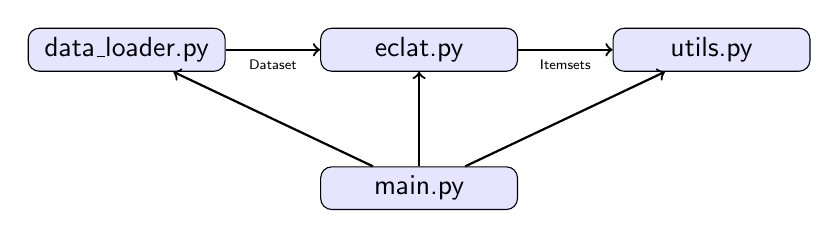
\begin{tikzpicture}[node distance=1.2cm, box/.style={rectangle, draw, rounded corners, fill=blue!10, text centered, minimum width=2.5cm}]
        \node[box] (data) {data\_loader.py};
        \node[box, right=of data] (algo) {eclat.py};
        \node[box, right=of algo] (utils) {utils.py};
        \node[box, below=of algo] (main) {main.py};
        
        \draw[->, thick] (main) -- (data);
        \draw[->, thick] (main) -- (algo);
        \draw[->, thick] (main) -- (utils);
        \draw[->, thick] (data) -- (algo) node[midway, below]{\tiny Dataset};
        \draw[->, thick] (algo) -- (utils) node[midway, below]{\tiny Itemsets};
    \end{tikzpicture}
    
    \vspace{0.5cm}
    \begin{itemize}
        \item \textbf{data\_loader.py}: Đọc và tiền xử lý dữ liệu.
        \item \textbf{eclat.py}: Cài đặt class Eclat và thuật toán đệ quy.
        \item \textbf{utils.py}: Sinh luật từ tập phổ biến.
        \item \textbf{main.py}: File chạy chính.
    \end{itemize}
\end{frame}

\begin{frame}[fragile]{Cài đặt Eclat (Python)}
    \begin{lstlisting}
def _eclat_recursive(self, prefix, items, min_sup):
    while items:
        # Lay item dau tien (Pop)
        item, tids = items.pop(0)
        new_itemset = prefix + [item]
        
        # Luu ket qua
        if len(new_itemset) >= self.min_items:
            self.frequent_itemsets.append((new_itemset, len(tids)))
        
        # Tao danh sach ung vien tiep theo (Intersection)
        next_items = []
        for other_item, other_tids in items:
            new_tids = tids & other_tids  # Giao
            
            if len(new_tids) >= min_sup:  # Cat tia
                next_items.append((other_item, new_tids))
        
        # De quy DFS
        if next_items:
            self._eclat_recursive(new_itemset, next_items, min_sup)
    \end{lstlisting}
\end{frame}
% (End of Implementation section)
    


% ============================================================
% CHƯƠNG 5: KẾT QUẢ VÀ ĐÁNH GIÁ
% ============================================================
\section{Kết quả và đánh giá}

\begin{frame}{Cấu hình và Kết quả tổng quan}
    \textbf{Cấu hình thực nghiệm:}
    \begin{itemize}
        \item Dữ liệu: Toàn bộ 989,818 phiên.
        \item Min Support: \textbf{0.02 (2\%)}.
        \item Min Confidence: \textbf{0.40 (40\%)}.
    \end{itemize}

    \vspace{0.3cm}
    \textbf{Kết quả:}
    \begin{itemize}
        \item 1-itemsets phổ biến: 15/17.
        \item 2-itemsets phổ biến: 17 cặp.
        \item \textbf{Tổng số tập phổ biến: 32}.
    \end{itemize}
    


\end{frame}


% --- KẾT QUẢ KHAI PHÁ LUẬT ---

\begin{frame}{Top 5 Luật gợi ý mạnh nhất}
    \begin{table}
    \centering\footnotesize
    \begin{tabular}{|c|l|l|c|c|c|}
    \hline
    \textbf{\#} & \textbf{Nếu xem} & \textbf{Gợi ý} & \textbf{Support} & \textbf{Conf.} & \textbf{Lift} \\
    \hline
    1 & Tổng hợp & Phát sóng & 3.36\% & 41.3\% & \textbf{1.88} \\
    2 & Kinh doanh & Trang chủ & 3.31\% & \textbf{56.8\%} & 1.80 \\
    3 & Đời sống & Trang chủ & 2.65\% & 51.9\% & 1.64 \\
    4 & Tổng hợp & Trang chủ & 3.68\% & 45.2\% & 1.43 \\
    5 & Tin tức & Trang chủ & 7.55\% & 42.6\% & 1.35 \\
    \hline
    \end{tabular}
    \end{table}
    
    \textit{(Đã lọc lift > 1 để đảm bảo tương quan dương)}
\end{frame}

\begin{frame}{Phân tích chi tiết}
    \textbf{1. Luật: Tổng hợp $\Rightarrow$ Phát sóng (Lift = 1.88)}
    \begin{itemize}
        \item \textbf{Insight}: Người xem tin tổng hợp rất thích xem video (Phát sóng). Xác suất xem video tăng gấp \textbf{1.88 lần} nếu họ đang ở mục Tổng hợp.
        \item \textbf{Gợi ý}: Nhúng widget Video vào trang Tổng hợp.
    \end{itemize}

    \vspace{0.3cm}
    \textbf{2. Luật: Kinh doanh $\Rightarrow$ Trang chủ (Conf = 56.8\%)}
    \begin{itemize}
        \item \textbf{Insight}: Hơn một nửa người đọc tin Kinh doanh sẽ quay lại Trang chủ.
        \item \textbf{Gợi ý}: Đặt nút "Về trang chủ" nổi bật hoặc banner tin nóng trên trang Kinh doanh.
    \end{itemize}
\end{frame}

% --- THỰC NGHIỆM SO SÁNH ---

\begin{frame}{Thực nghiệm: So sánh Eclat và Apriori}
    \textbf{Mục tiêu:} Chứng minh hiệu quả của Eclat so với thuật toán truyền thống Apriori trên cùng bộ dữ liệu.
    
    \vspace{0.2cm}
    \textbf{Thiết lập thực nghiệm:}
    \begin{itemize}
        \item \textbf{Dữ liệu}: \textbf{Toàn bộ 989,818 phiên giao dịch} (MSNBC.com).
        \item \textbf{Tham số}: Min Support thay đổi từ 5\% xuống 1\%.
        \item \textbf{Môi trường}: Python 3.x, chạy trên cùng một máy tính.
    \end{itemize}

    \vspace{0.2cm}
    \textbf{Kết quả đo lường (Tại Min Support = 1\%):}
    \begin{table}\centering\small
    \begin{tabular}{|l|c|c|}
    \hline
    \textbf{Thuật toán} & \textbf{Thời gian (s)} & \textbf{Bộ nhớ đỉnh (MB)} \\
    \hline
    \textbf{Apriori} & 15.62s & \textbf{0.04 MB} \\
    \hline
    \textbf{Eclat} & \textbf{2.16s} & 111.81 MB \\
    \hline
    \textbf{Kết luận} & \textbf{Nhanh hơn $\approx$ 7 lần} & Tốn bộ nhớ hơn \\
    \hline
    \end{tabular}
    \end{table}
\end{frame}

\begin{frame}{Biểu đồ so sánh hiệu năng}
    \begin{figure}
        \centering
        \includegraphics[width=1.0\textwidth]{images/comparison_chart.png}
        \caption{So sánh Thời gian thực thi và Bộ nhớ sử dụng giữa Apriori và Eclat}
    \end{figure}
    
    \textbf{Nhận xét:}
    \begin{itemize}
        \item \textbf{Thời gian}: Eclat nhanh hơn đáng kể khi Support giảm (dữ liệu phức tạp hơn) nhờ không phải quét lại CSDL.
        \item \textbf{Bộ nhớ}: Eclat tốn nhiều RAM hơn để lưu trữ cấu trúc TID-Sets (Vertical Format), đây là sự đánh đổi (Trade-off) để lấy tốc độ.
    \end{itemize}
\end{frame}

% ============================================================
% CHƯƠNG 6: KẾT LUẬN
% ============================================================
\section{Kết luận}

\begin{frame}{Tổng kết}
    Đề tài đã đạt được các mục tiêu:
    \begin{itemize}
        \item[$\checkmark$] Hiểu và cài đặt thành công thuật toán \textbf{Eclat} (DFS, Vertical Format).
        \item[$\checkmark$] Xử lý hiệu quả tập dữ liệu lớn (~1 triệu dòng) từ MSNBC.
        \item[$\checkmark$] Tìm ra các luật có ý nghĩa (Lift > 1) để ứng dụng gợi ý nội dung.
    \end{itemize}
\end{frame}

\begin{frame}{Hạn chế và Hướng phát triển}
    \textbf{Hạn chế:}
    \begin{itemize}
        \item Dữ liệu cũ (1999), chưa phản ánh trends hiện tại.
        \item Thuật toán Eclat tiêu tốn nhiều bộ nhớ hơn (RAM) do lưu trữ TID-Sets.
        \item Chưa xét đến \textbf{thứ tự} click (Sequential Mining) mà chỉ xét sự xuất hiện đồng thời.
    \end{itemize}

    \vspace{0.5cm}
    \textbf{Hướng phát triển:}
    \begin{itemize}
        \item \textbf{Sequential Mining}: Áp dụng GSP, PrefixSpan để xét đến \textit{thứ tự} click.
        \item \textbf{Real-time}: Tích hợp vào hệ thống gợi ý thời gian thực.
        \item \textbf{Demo}: Xây dựng giao diện Web App trực quan.
    \end{itemize}
\end{frame}

\begin{frame}
    \centering
    \Huge \textbf{CẢM ƠN THẦY VÀ CÁC BẠN\\ĐÃ LẮNG NGHE!}
    
    \vspace{1cm}
    \large \textbf{Q \& A}
\end{frame}

\end{document}
